L'intero lavoro di tesi è stato svolto in Python\cite{python}, utilizzando un notebook Jupyter\cite{jupyter} come ambiente di esecuzione.

Le librerie selezionate per il progetto sono state di fondamentale importanza per il raggiungimento degli obiettivi prefissati:
\begin{itemize}
    \item \textbf{pypdf}: Questa libreria è stata impiegata per l'estrazione accurata del testo da documenti in formato PDF, consentendo così di lavorare con il contenuto testuale essenziale.
    \item \textbf{pandas}: Essenziale per la gestione efficiente del file XLSX contenente i metadati dei documenti. La flessibilità di Pandas ha facilitato la manipolazione e l'analisi dei dati correlati.
    \item \textbf{tiktoken}: L'implementazione del byte pair encoding (BPE) e della tokenizzazione tramite Tiktoken è stata cruciale per la preparazione dei testi e la loro successiva elaborazione nei modelli di OpenAI. 
    \item \textbf{openai}: La libreria ufficiale di OpenAI è stata utilizzata per interagire con i modelli e le API di OpenAI, consentendo un'interazione agevole e l'integrazione dei risultati nei processi di analisi.
    \item \textbf{langchain}: Questa libreria, che può essere considerata a tutti gli effetti un framework, è stata il fulcro centrale del lavoro di tesi. Grazie ad essa è stato possibile arricchire le capacità di un large language model con concetti avanzati, i quali saranno dettagliatamente esposti in seguito.
    \item \textbf{chromadb}: L'utilizzo della libreria ufficiale di ChromaDB ha consentito la conservazione e l'efficace interrogazione dei vettori di embeddings, rappresentando un passo cruciale per l'analisi e l'elaborazione dei dati ottenuti.
\end{itemize}

Il notebook è stato eseguito su piattaforma Google Colab, che oltre all'esecuzione permette di accedere allo storage di google drive, dove è stato conservato il dataset, in modo semplice e veloce come se fosse una directory della macchina in cui gira il notebook.

L'attenta scelta e l'integrazione di queste librerie hanno fornito gli strumenti necessari per l'elaborazione accurata e la valorizzazione dei dati, contribuendo significativamente al raggiungimento degli obiettivi di ricerca.

L'implementazione del progetto è stata suddivisa in due fasi principali: ingestion e inferenza.

\subsection{Ingestion} 
La fase di ingestion dei dati è descritta dal diagramma di flusso in figura 4.1:
\begin{figure}[H]
    \centering
    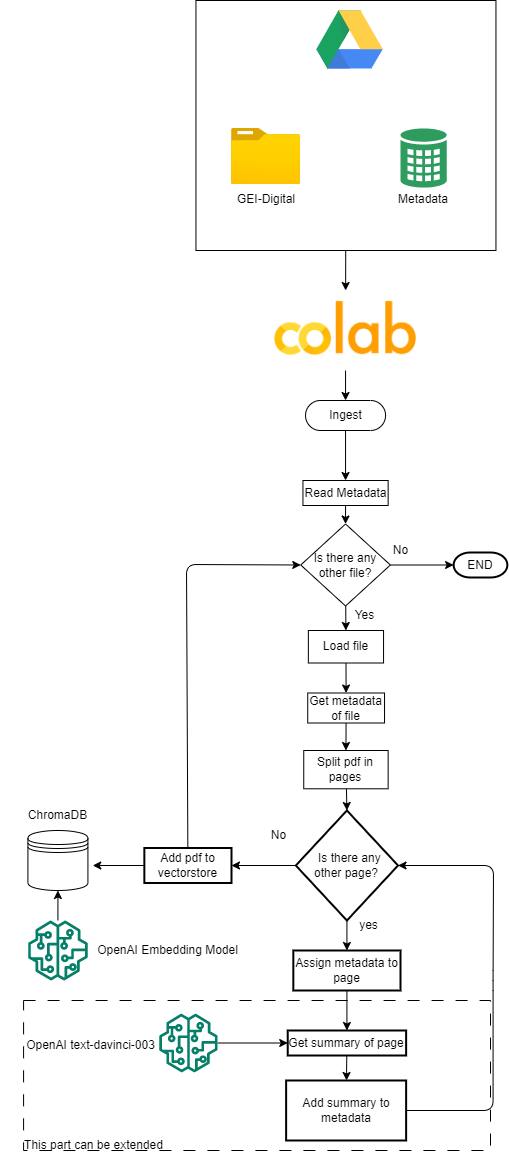
\includegraphics[height=0.5\pdfpageheight]{images/ingest.png}\label{fig:ingest}
    \caption[Ingestion]{Il diagramma di flusso che descrive la fase di ingest dei dati.}
\end{figure}

Come si può osservare, i dati sono stati conservati su Google Drive e il job di ingestion si occupa di leggere i 33 libri in formato pdf,
suddividerli in pagine assegnando loro le informazioni derivanti dai metadati, è presente inoltre una parte di enrichment di tali informazioni 
utilizzando il Large Language Model ``text-davinci-003'' di OpenAI per estrarre un riassunto di ogni pagina. Quest'ultima parte di enrichment è possibile espanderla ulteriormente
utilizzando l'LLM per estrarre ulteriori informazioni, come ad esempio le entità presenti in ogni pagina, ma per il momento è stata tralasciata.

Alimentato il database con le informazioni estratte, è possibile passare alla fase di inferenza.

\subsection[Inferenza]{Inferenza e interazione con l'utente}

La fase di inferenza e interazione con l'utente è descritta dal diagramma di flusso in figura 4.2:

\begin{figure}[H]
    \centering
    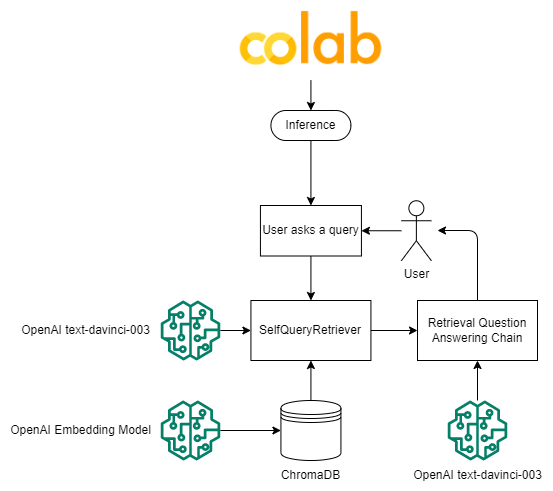
\includegraphics[height=0.3\pdfpageheight]{images/Inference.png}\label{fig:infer}
    \caption[Ingestion]{Il diagramma di flusso che descrive l'interazione dell'utente con il sistema di question answering.}
\end{figure}

\lipsum[1-4]